\chapter{Aesthetic Analysis}\label{ch:aesthetics}

\section{Placement of Floats}
Since all text layout is precomputed, the only remaining concern is that the columns of text and floats are laid out in a pleasing manner. Plass~\cite{Plass1981} devised a system to perform optimal placement of floats within text, whereby float placement is penalised by the square of the distance from its intended position. He showed that this problem was NP-hard, but he also showed that a similar (but less ``optimal'') system using linear penalties could be made computationally tractable.

Br\"uggemann-Klein et al.~\cite{Bruggemann-Klein1995} suggested that Plass's method is only optimal for a given definition of ``optimal''. They proposed that a superior metric for float placement is to minimise the number of page turns that a reader must perform when reading the document from front to back. This is a desirable characteristic for a pagination algorithm that runs on an \ebook{} reader, because page turns tend to be slow, particularly on devices with electronic paper displays. Unfortunately, the algorithm used runs in quadratic time, which limits its usefulness to this system.

In essence, the assumption that Plass's float placement algorithm produces the most optimal layouts may be slightly short-sighted: \emph{other pagination schemes are available!} Clearly, using a computationally intractable algorithm such as Plass's will have significant impact on the demand for computation at view-time. As with many facets of the system described in this thesis, the float placement algorithm was chosen with efficiency in mind.

The float placement algorithm that has been developed for use with the malleable document system also attempts to minimise the distance between the actual and intended positioning of floats: if a float can be placed directly at its intended position, then it will be, otherwise it will be placed in the next available space. (Figure~\ref{fig:gridlayout} on page~\pageref{fig:gridlayout} demonstrates this process.)

Whilst this algorithm does not perform any lookahead or backtracking in order to place floats optimally, experiments have shown that in most cases, floats are placed directly in their intended positions or at the top of adjacent columns, and are only occasionally moved across page boundaries. Figures \ref{fig:example-portrait}, \ref{fig:example-landscape}, and~\ref{fig:example-ereader} show some examples of layouts produced using this algorithm, and Figures \ref{fig:example-latex} and~\ref{fig:example-html} show some comparative renderings of the same document, produced by \LaTeX{} and a web browser respectively. The output of the malleable document system looks very similar to that of \LaTeX, and very different from that of the web browser.

As it stands, the algorithm does not avoid widowed or orphaned lines, nor single lines directly before or after floats. This can be seen clearly in Figure~\ref{fig:example-ereader} at the top of the fourth page, where the float has spanned both columns and taken up all the space on the page, with the exception of one line at the top of each column. It would not be too difficult to add a constraint that states that single lines of text at the top or bottom of the page should never be allowed, which could be enforced by leaving extra lines blank, pushing the text forward, though it is possible that this may harm the balance of the page if it causes columns to have uneven lengths.

\begin{figure}
\begin{center}
\fbox{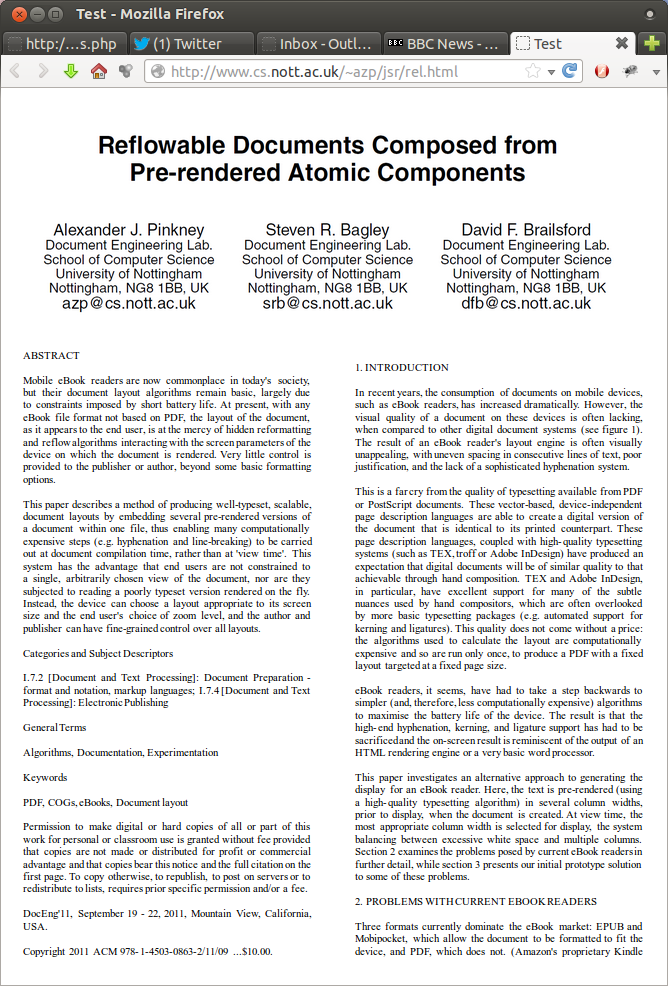
\includegraphics[trim=0in 0in 0in 1.2in, clip=true, width=0.47\textwidth]{gfx/p1}}\hspace{0.01\textwidth}
\fbox{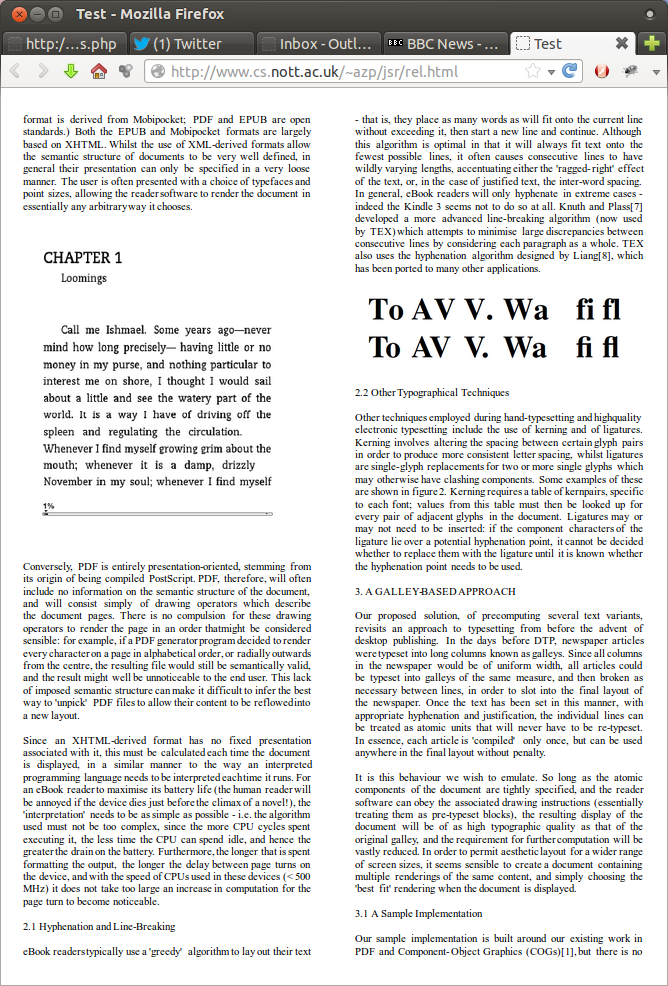
\includegraphics[trim=0in 0in 0in 1.2in, clip=true, width=0.47\textwidth]{gfx/p2}}

\vspace{0.2in}
\fbox{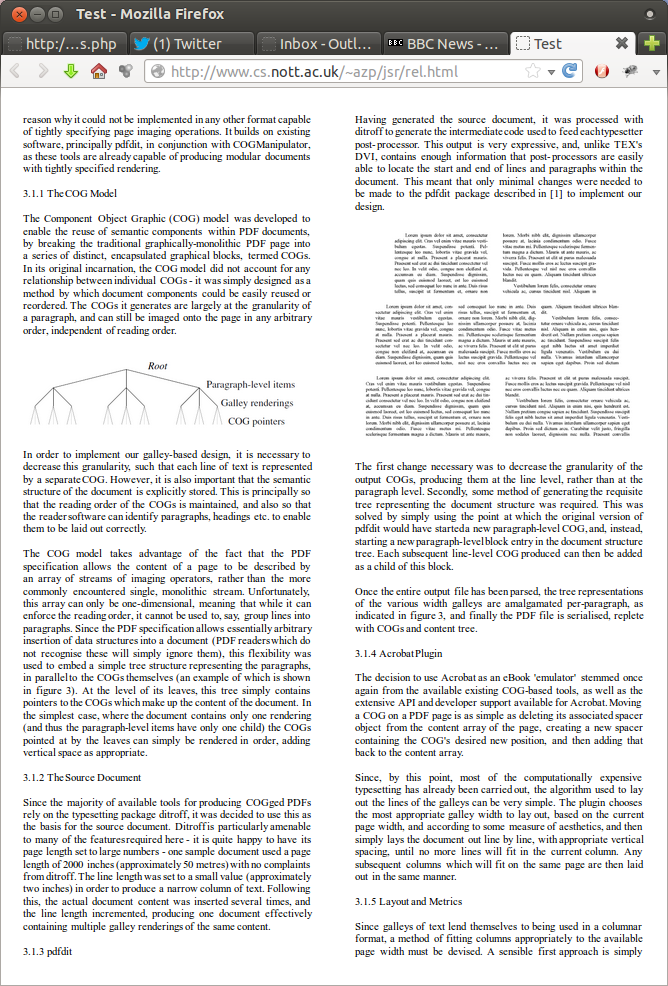
\includegraphics[trim=0in 0in 0in 1.2in, clip=true, width=0.47\textwidth]{gfx/p3}}\hspace{0.01\textwidth}
\fbox{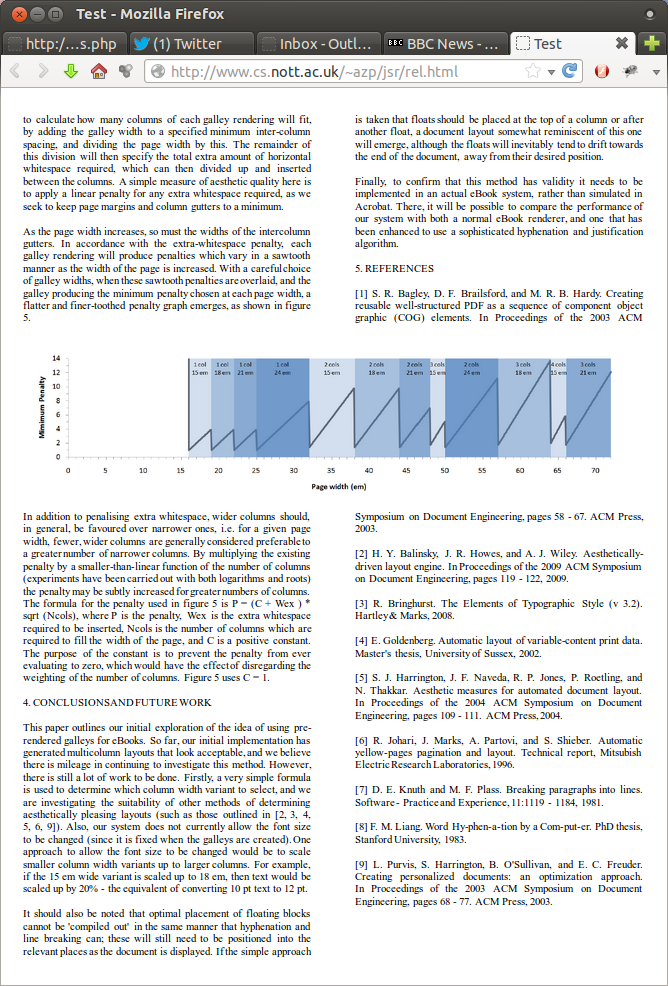
\includegraphics[trim=0in 0in 0in 1.2in, clip=true, width=0.47\textwidth]{gfx/p4}}
\end{center}
\caption[A sample of document layout]{\cite{Pinkney2011} laid out by the malleable document system, running in Mozilla Firefox. The page size has been selected to resemble that of A4 paper in a portrait orientation.}
\label{fig:example-portrait}
\end{figure}

\begin{sidewaysfigure}
\begin{center}
\fbox{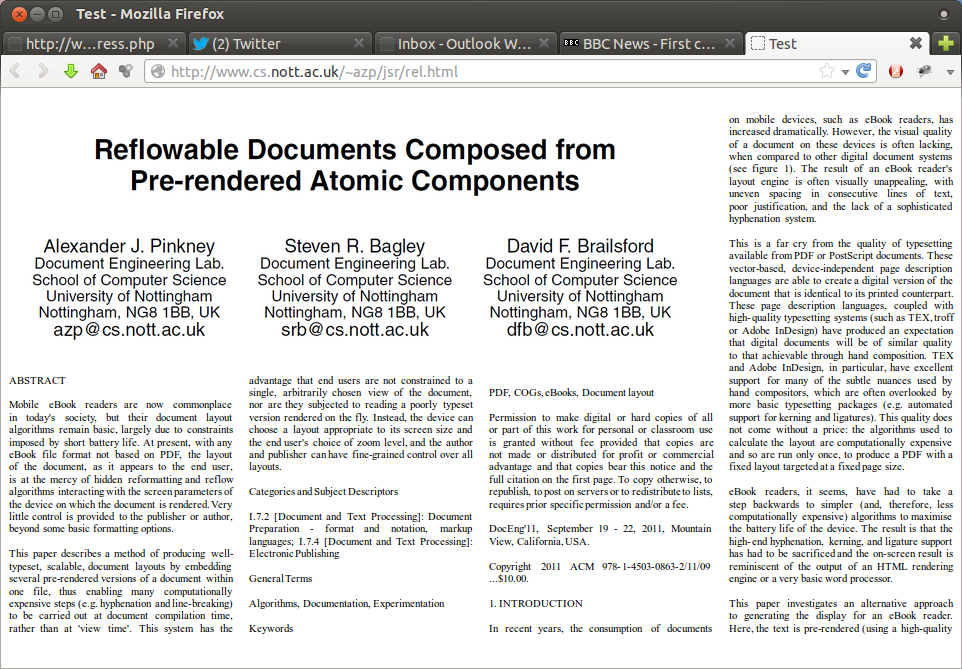
\includegraphics[trim=0in 0in 0in 1.2in, clip=true, width=0.45\textwidth]{gfx/q1}}\hspace{0.05\textwidth}
\fbox{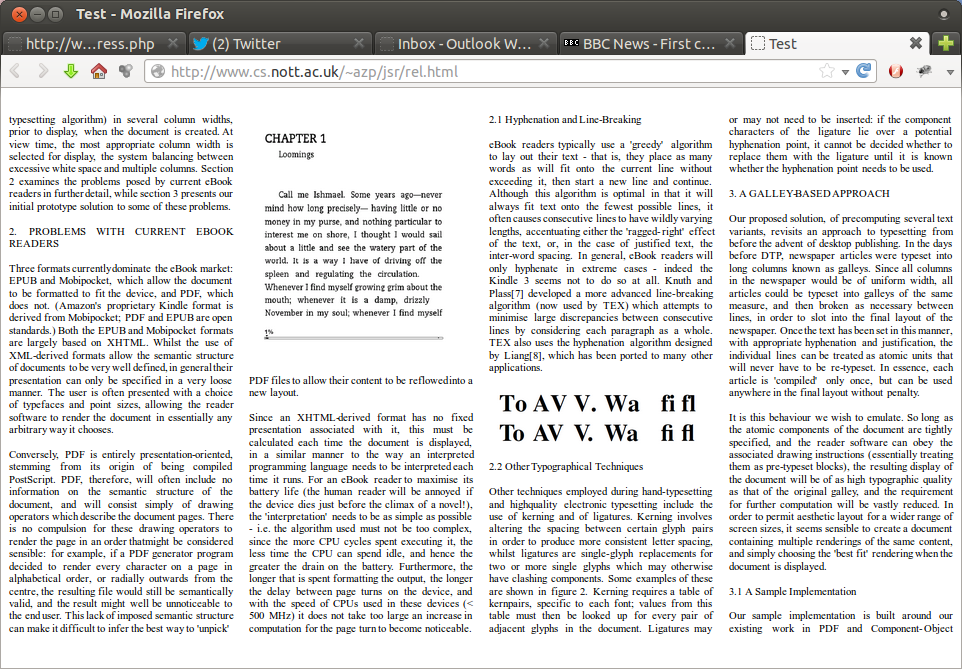
\includegraphics[trim=0in 0in 0in 1.2in, clip=true, width=0.45\textwidth]{gfx/q2}}

\vspace{0.2in}
\fbox{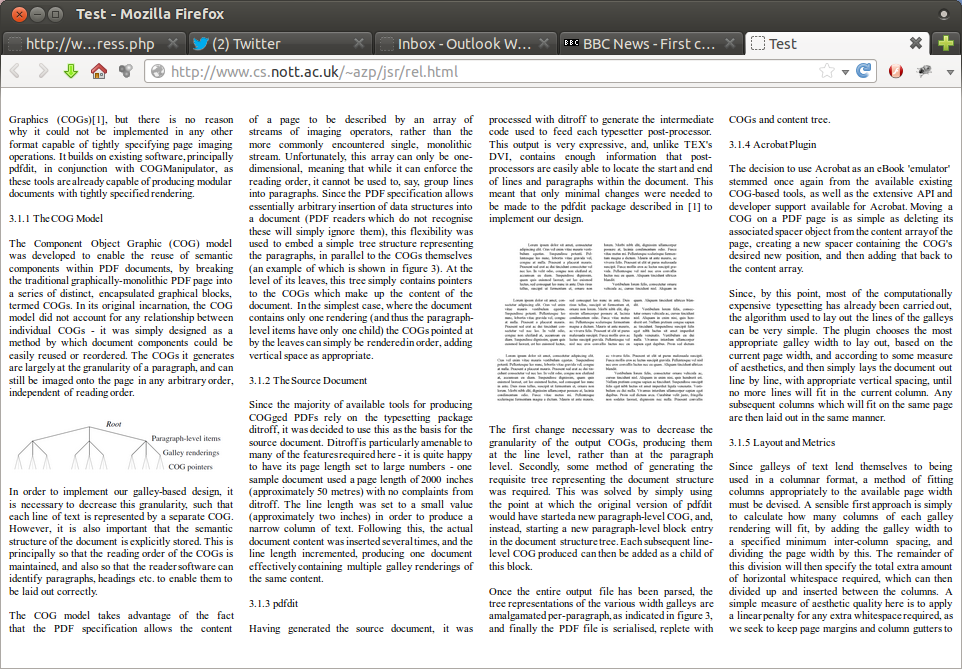
\includegraphics[trim=0in 0in 0in 1.2in, clip=true, width=0.45\textwidth]{gfx/q3}}\hspace{0.05\textwidth}
\fbox{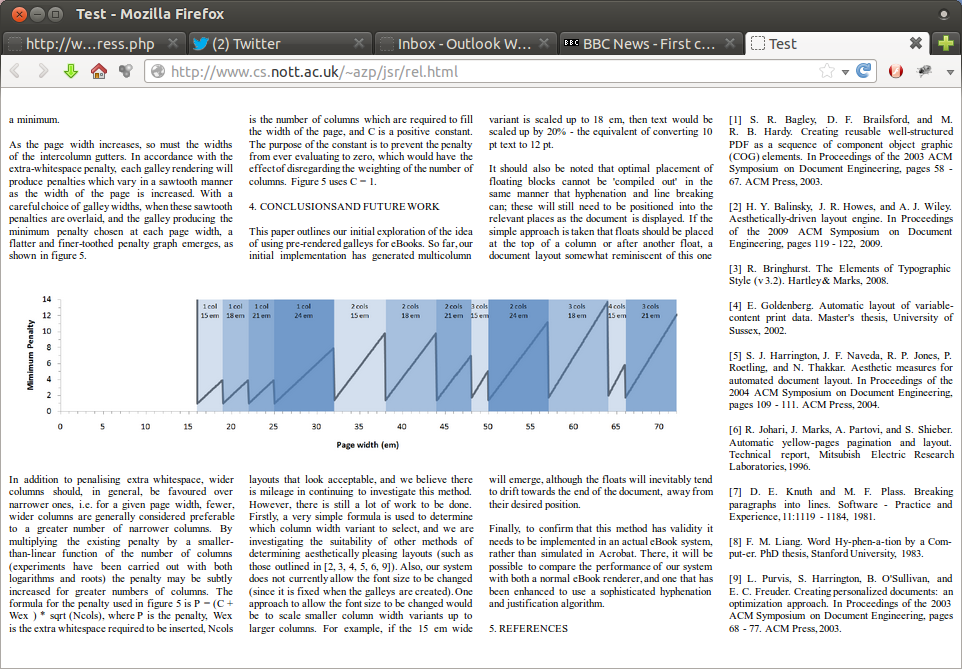
\includegraphics[trim=0in 0in 0in 1.2in, clip=true, width=0.45\textwidth]{gfx/q4}}
\end{center}
\caption[A sample of document layout]{\cite{Pinkney2011} laid out by the malleable document system, running in Mozilla Firefox. The page size has been selected to resemble that of A4 paper in a landscape orientation.}
\label{fig:example-landscape}
\end{sidewaysfigure}

\begin{figure}
\begin{center}
\newlength{\imgwid} \setlength{\imgwid}{0.29\textwidth}
\fbox{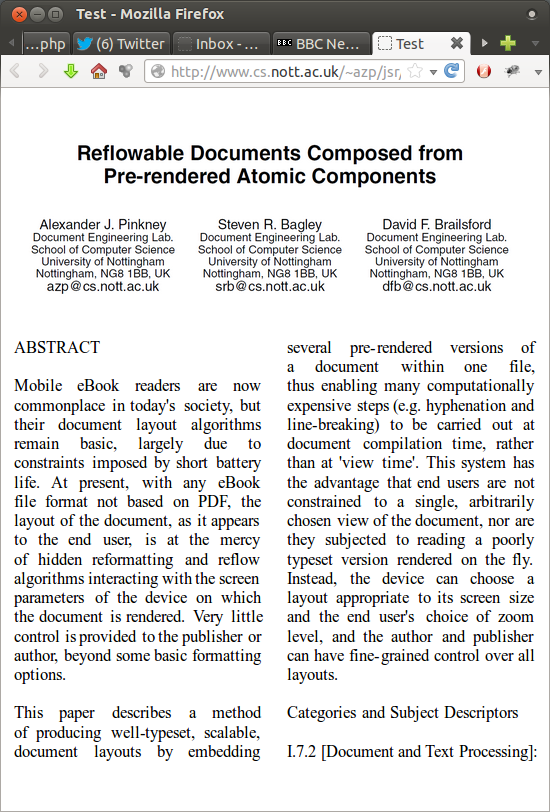
\includegraphics[trim=0in 0in 0in 1.2in, clip=true, width=\imgwid]{gfx/r1}}
\fbox{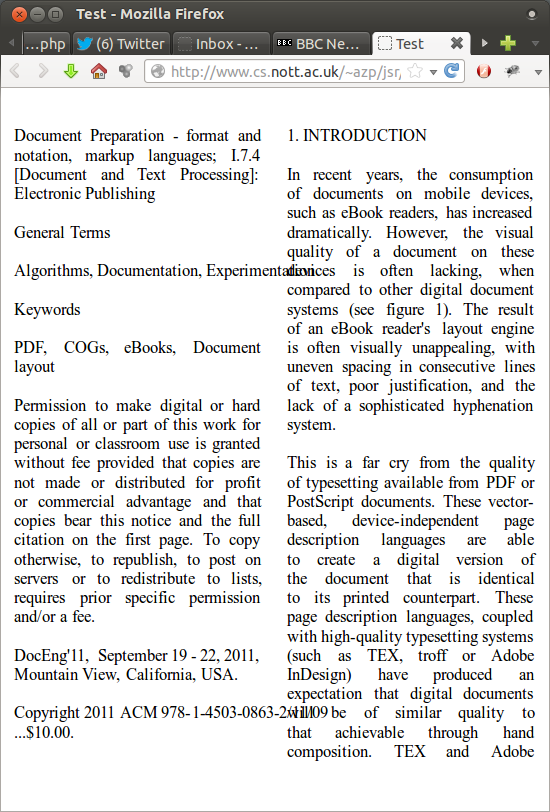
\includegraphics[trim=0in 0in 0in 1.2in, clip=true, width=\imgwid]{gfx/r2}}
\fbox{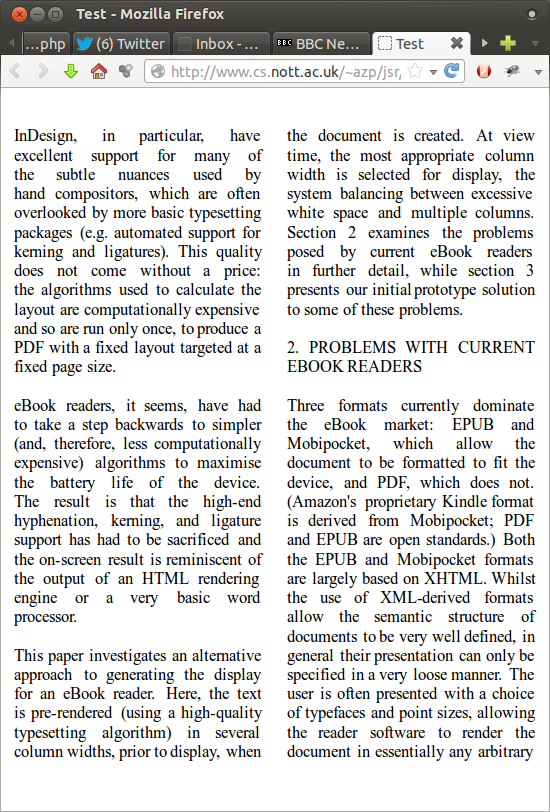
\includegraphics[trim=0in 0in 0in 1.2in, clip=true, width=\imgwid]{gfx/r3}}
\fbox{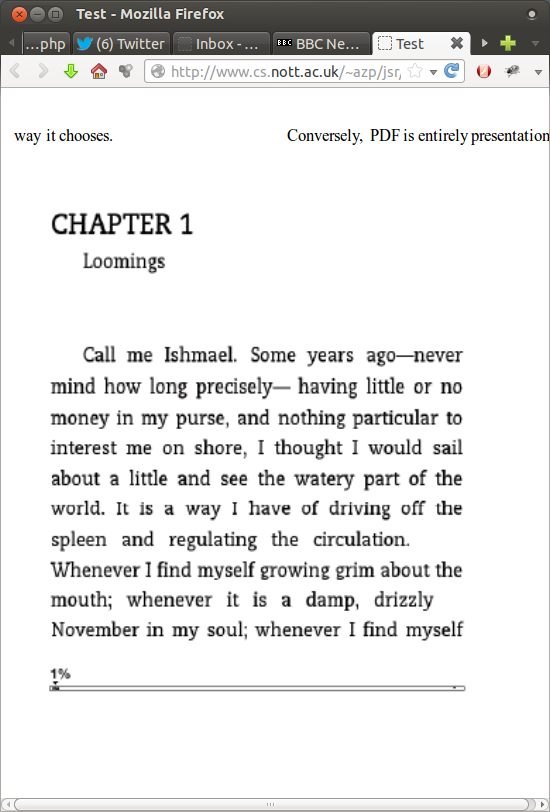
\includegraphics[trim=0in 0in 0in 1.2in, clip=true, width=\imgwid]{gfx/r4}}
\fbox{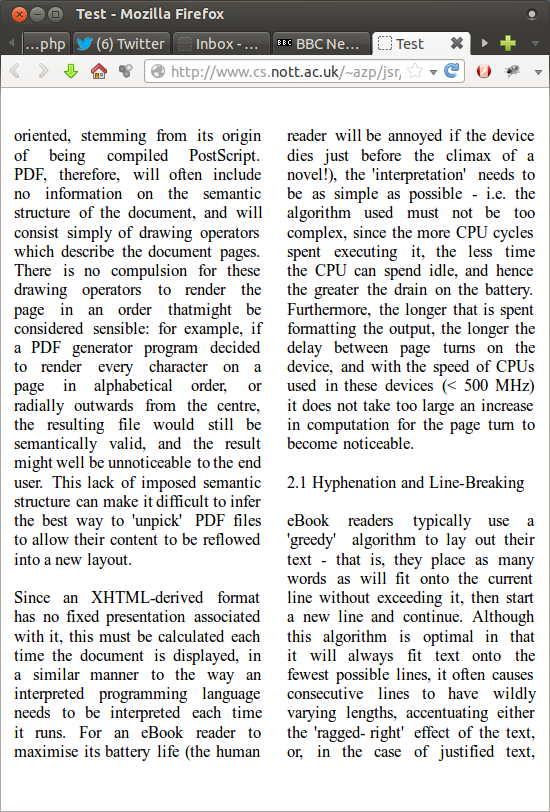
\includegraphics[trim=0in 0in 0in 1.2in, clip=true, width=\imgwid]{gfx/r5}}
\fbox{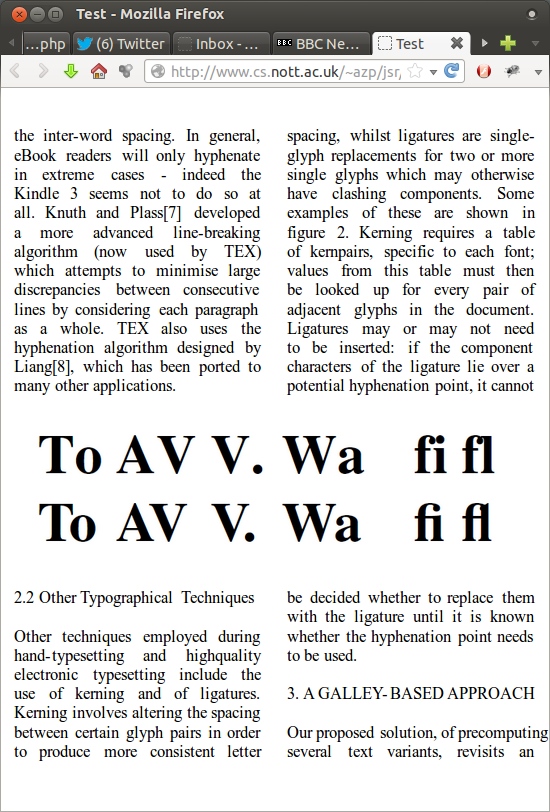
\includegraphics[trim=0in 0in 0in 1.2in, clip=true, width=\imgwid]{gfx/r6}}
\fbox{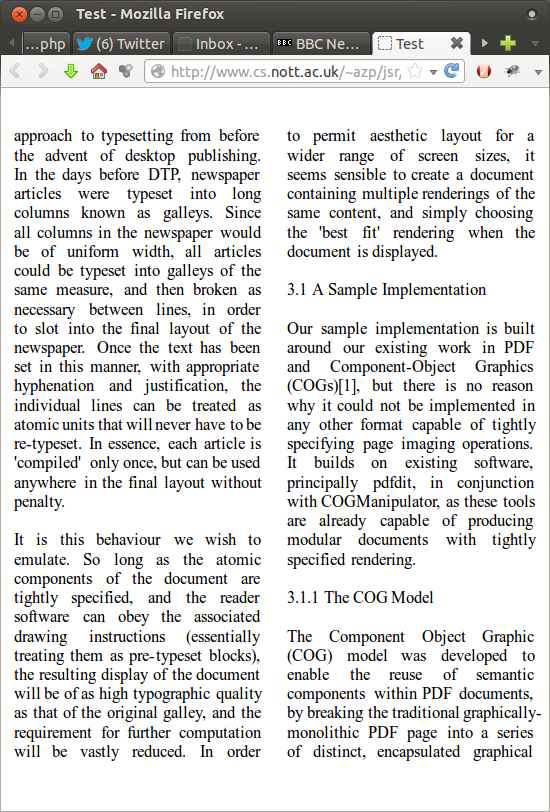
\includegraphics[trim=0in 0in 0in 1.2in, clip=true, width=\imgwid]{gfx/r7}}
\fbox{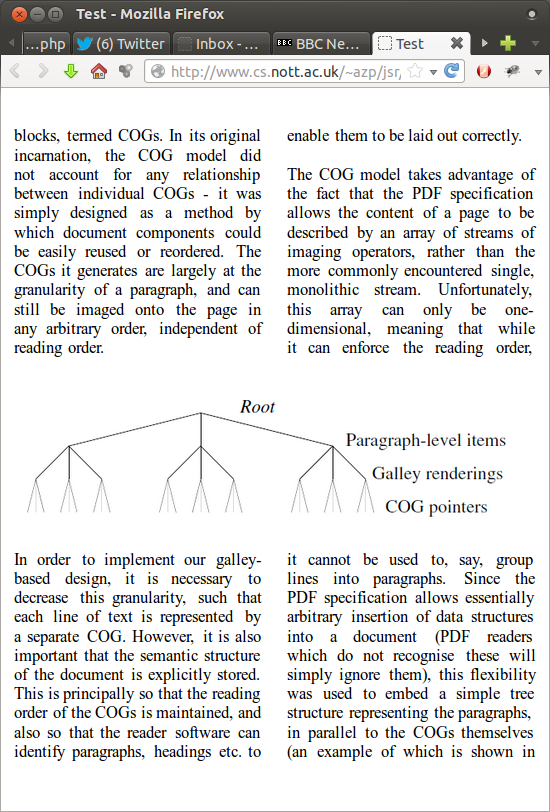
\includegraphics[trim=0in 0in 0in 1.2in, clip=true, width=\imgwid]{gfx/r8}}
\fbox{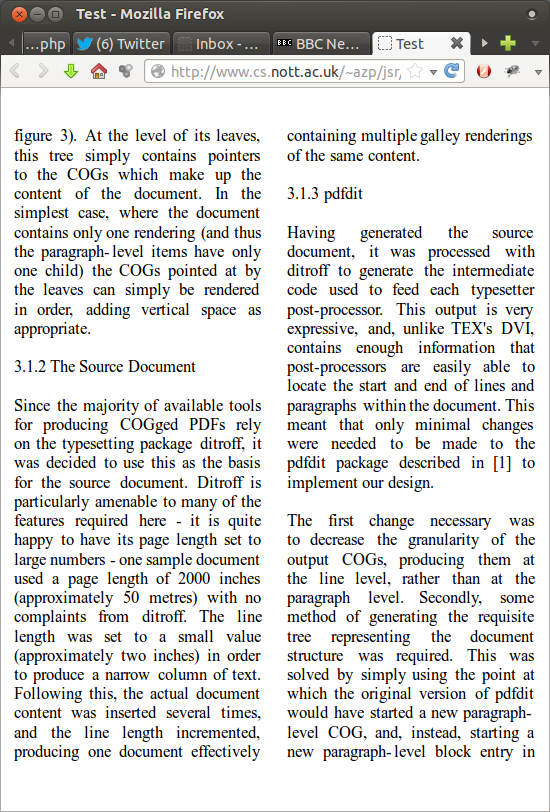
\includegraphics[trim=0in 0in 0in 1.2in, clip=true, width=\imgwid]{gfx/r9}}
\fbox{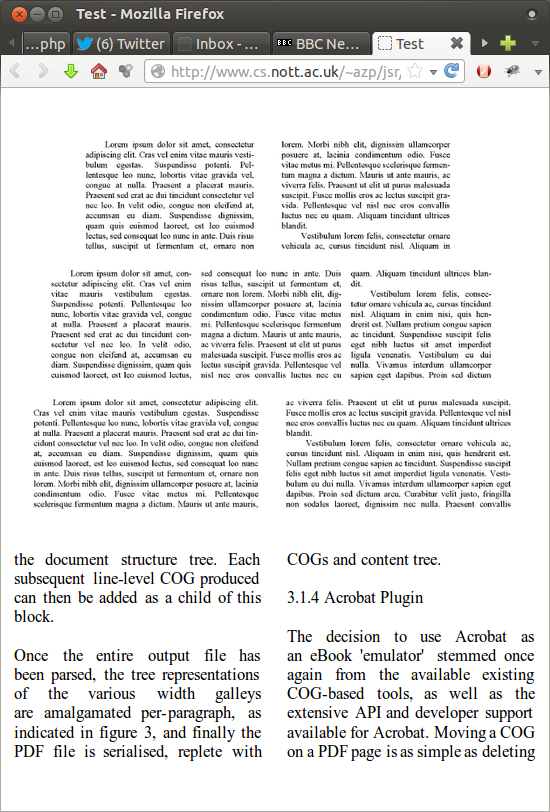
\includegraphics[trim=0in 0in 0in 1.2in, clip=true, width=\imgwid]{gfx/r10}}
\fbox{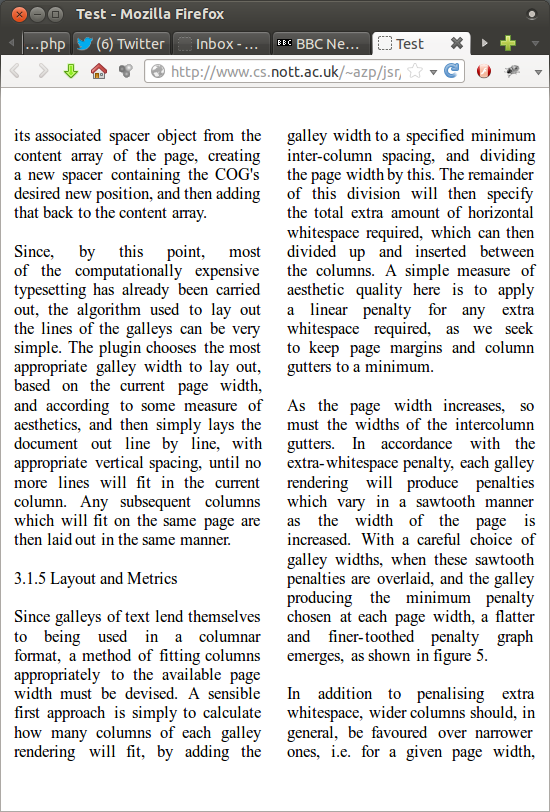
\includegraphics[trim=0in 0in 0in 1.2in, clip=true, width=\imgwid]{gfx/r11}}
\fbox{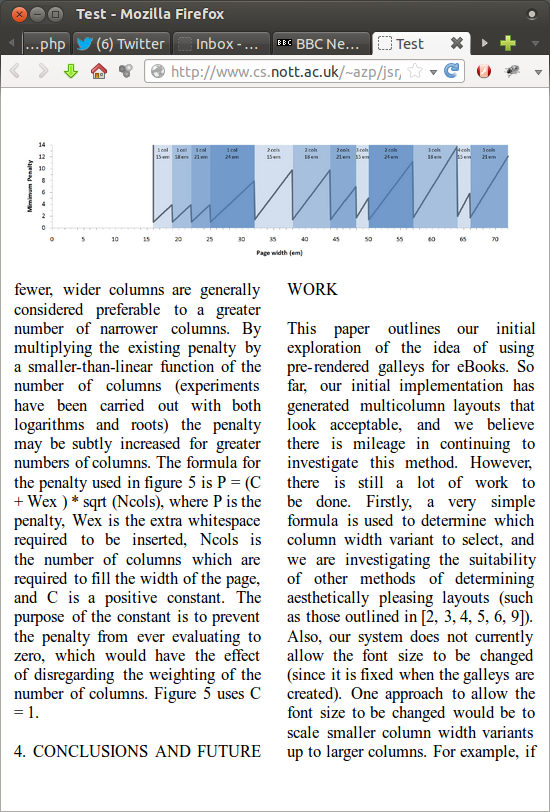
\includegraphics[trim=0in 0in 0in 1.2in, clip=true, width=\imgwid]{gfx/r12}}
\fbox{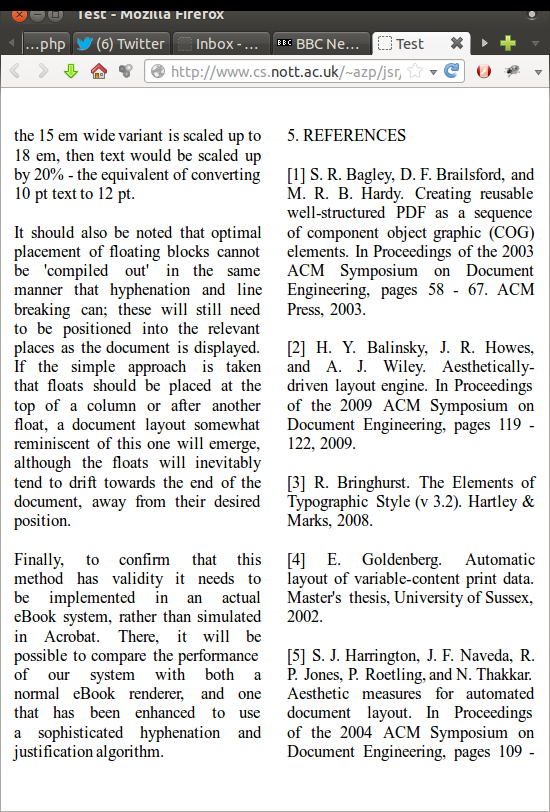
\includegraphics[trim=0in 0in 0in 1.2in, clip=true, width=\imgwid]{gfx/r13}}
\fbox{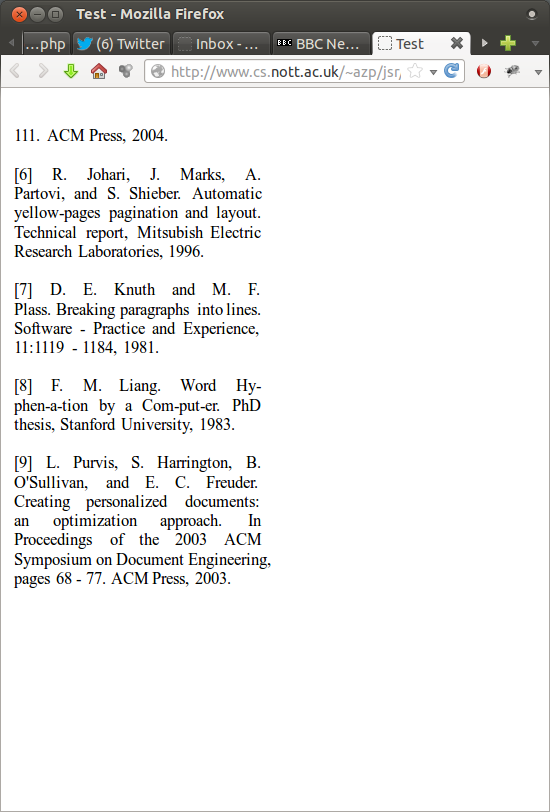
\includegraphics[trim=0in 0in 0in 1.2in, clip=true, width=\imgwid]{gfx/r14}}
\end{center}
\caption[A sample of document layout]{\cite{Pinkney2011} laid out by the malleable document system, running in Mozilla Firefox. The page size has been selected to resemble that of an \ebook{} reader in a portrait orientation.}
\label{fig:example-ereader}
\end{figure}

\begin{figure}
\begin{center}
\fbox{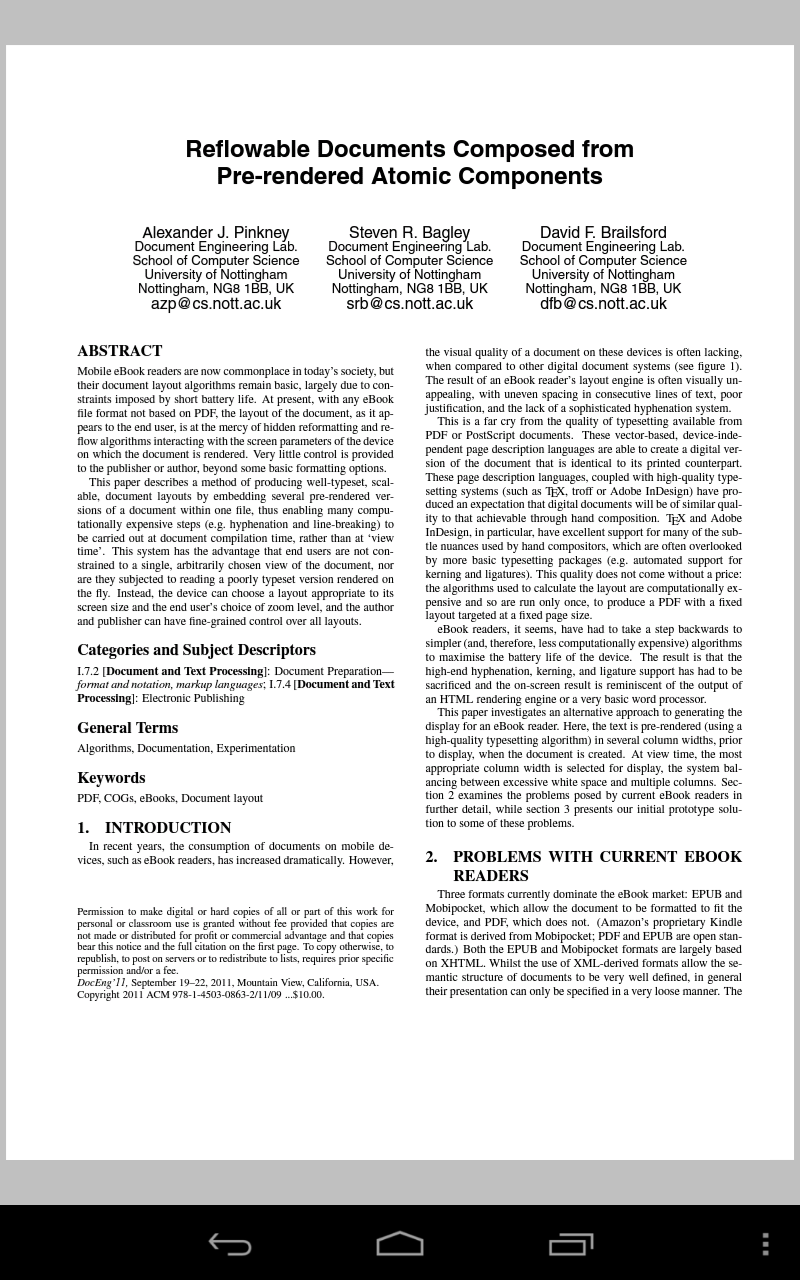
\includegraphics[trim=0.1in 2in 0.1in 1in, clip=true, width=0.47\textwidth]{gfx/pbb11-1}}\hspace{0.01\textwidth}
\fbox{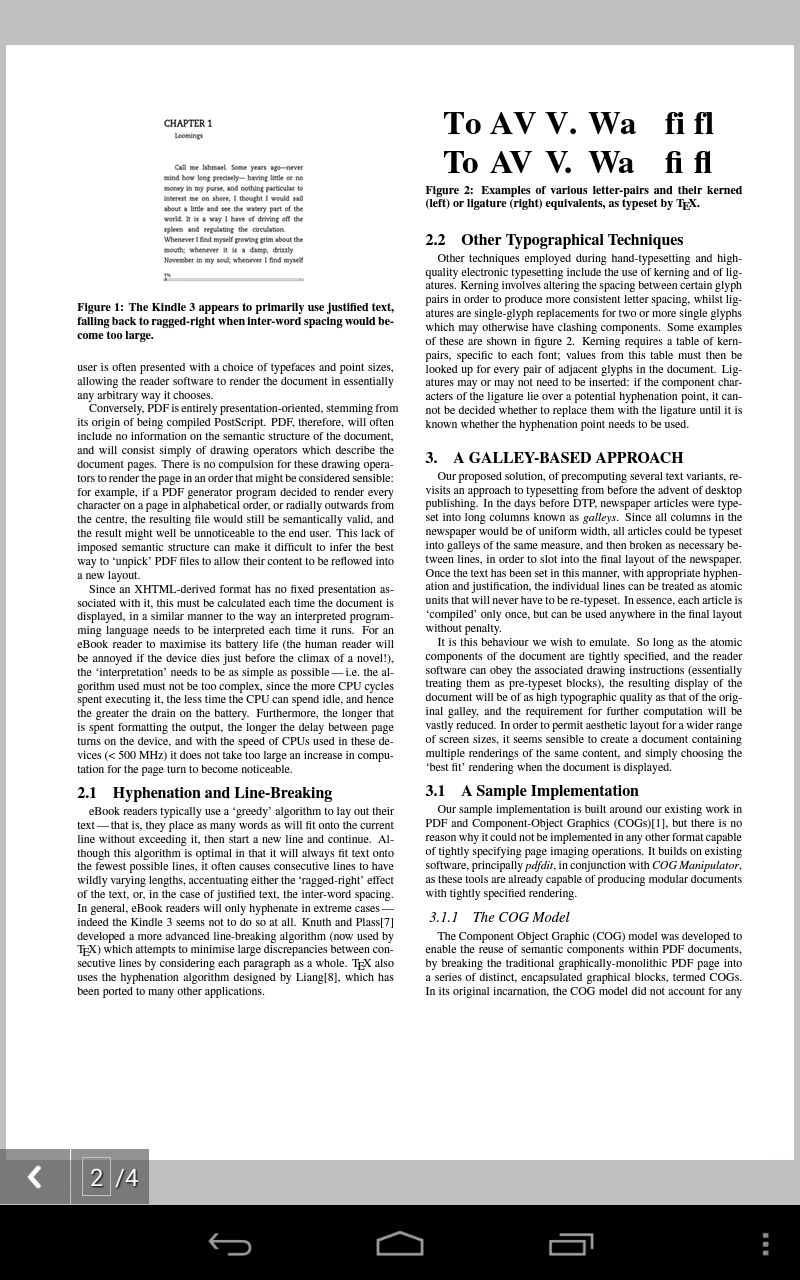
\includegraphics[trim=0.1in 2in 0.1in 1in, clip=true, width=0.47\textwidth]{gfx/pbb11-2}}

\vspace{0.2in}
\fbox{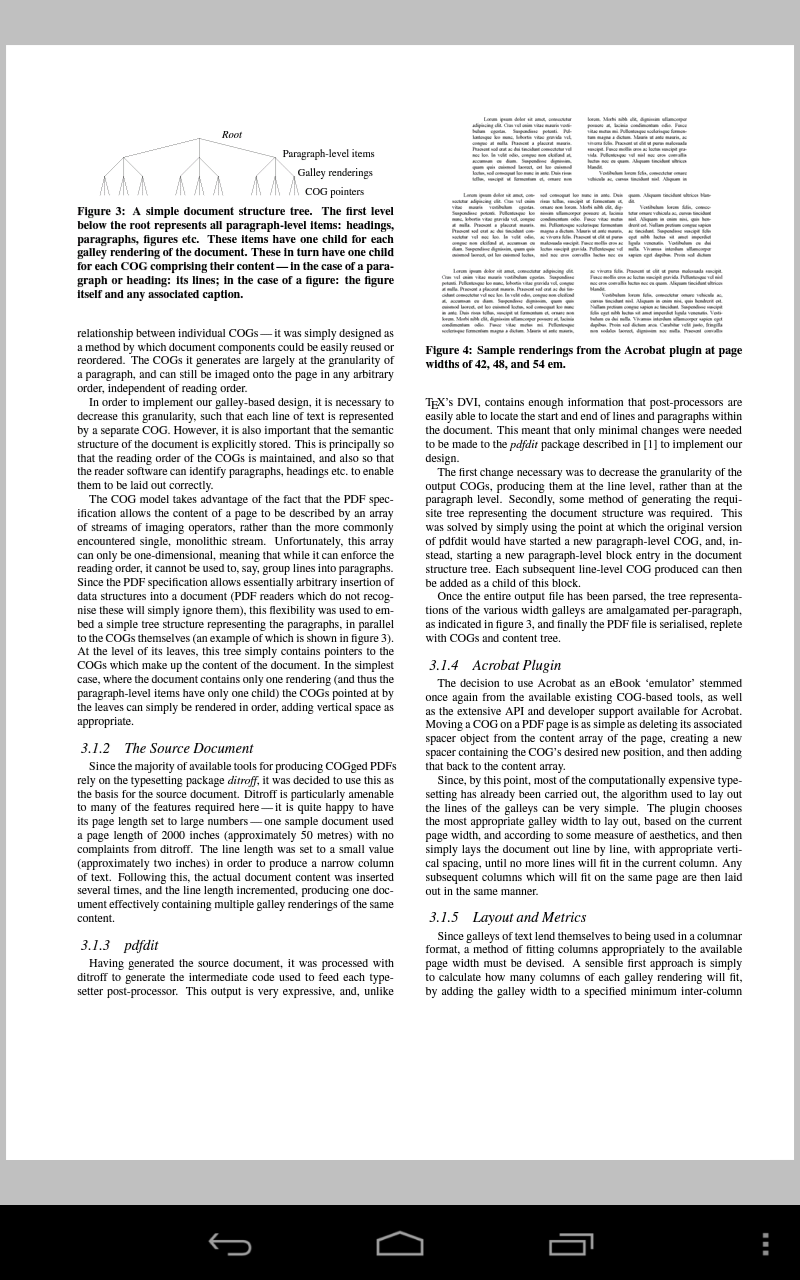
\includegraphics[trim=0.1in 2in 0.1in 1in, clip=true, width=0.47\textwidth]{gfx/pbb11-3}}\hspace{0.01\textwidth}
\fbox{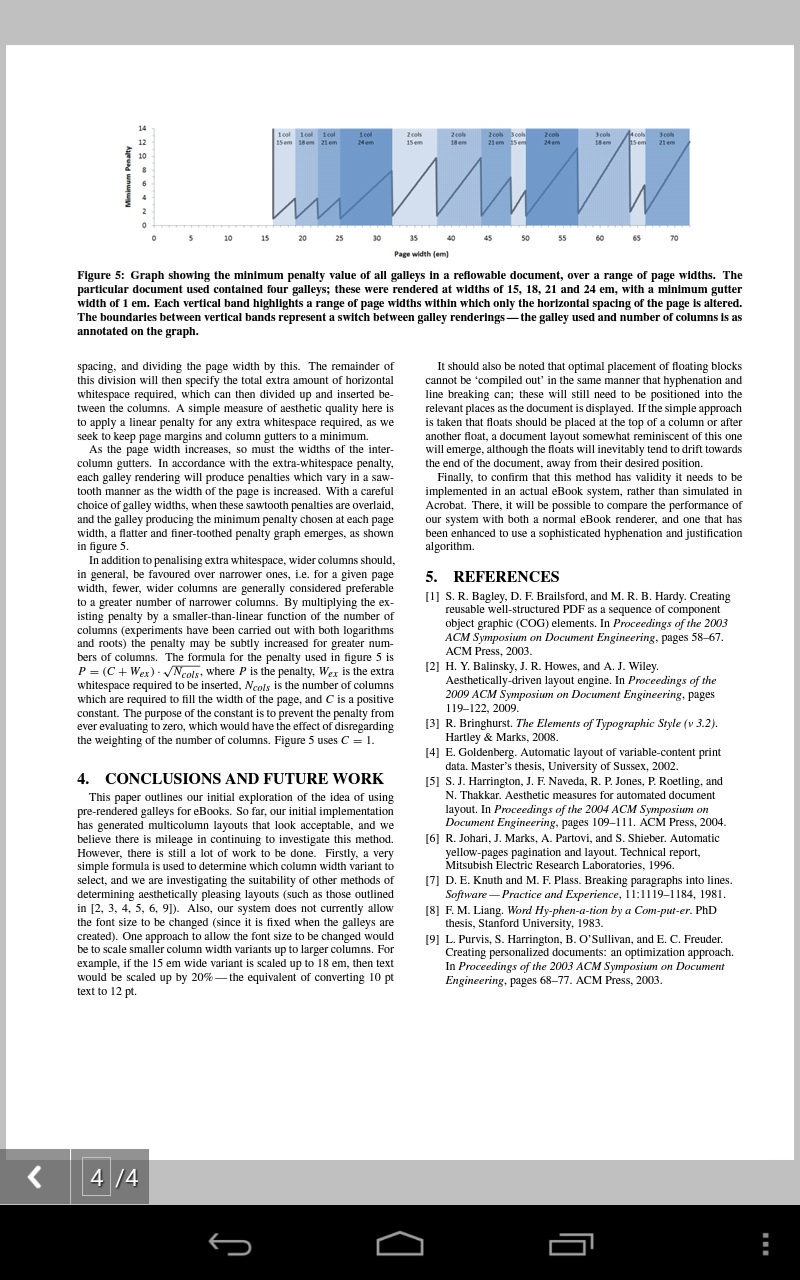
\includegraphics[trim=0.1in 2in 0.1in 1in, clip=true, width=0.47\textwidth]{gfx/pbb11-4}}
\end{center}
\caption[A document laid out by \LaTeX]{\cite{Pinkney2011} as rendered by \LaTeX. The layout is very similar to that shown in Figure~\ref{fig:example-portrait}, though \LaTeX{} favours placing floats at the top of columns, rather than directly at their logical position.}
\label{fig:example-latex}
\end{figure}

\begin{figure}
\begin{center}
\fbox{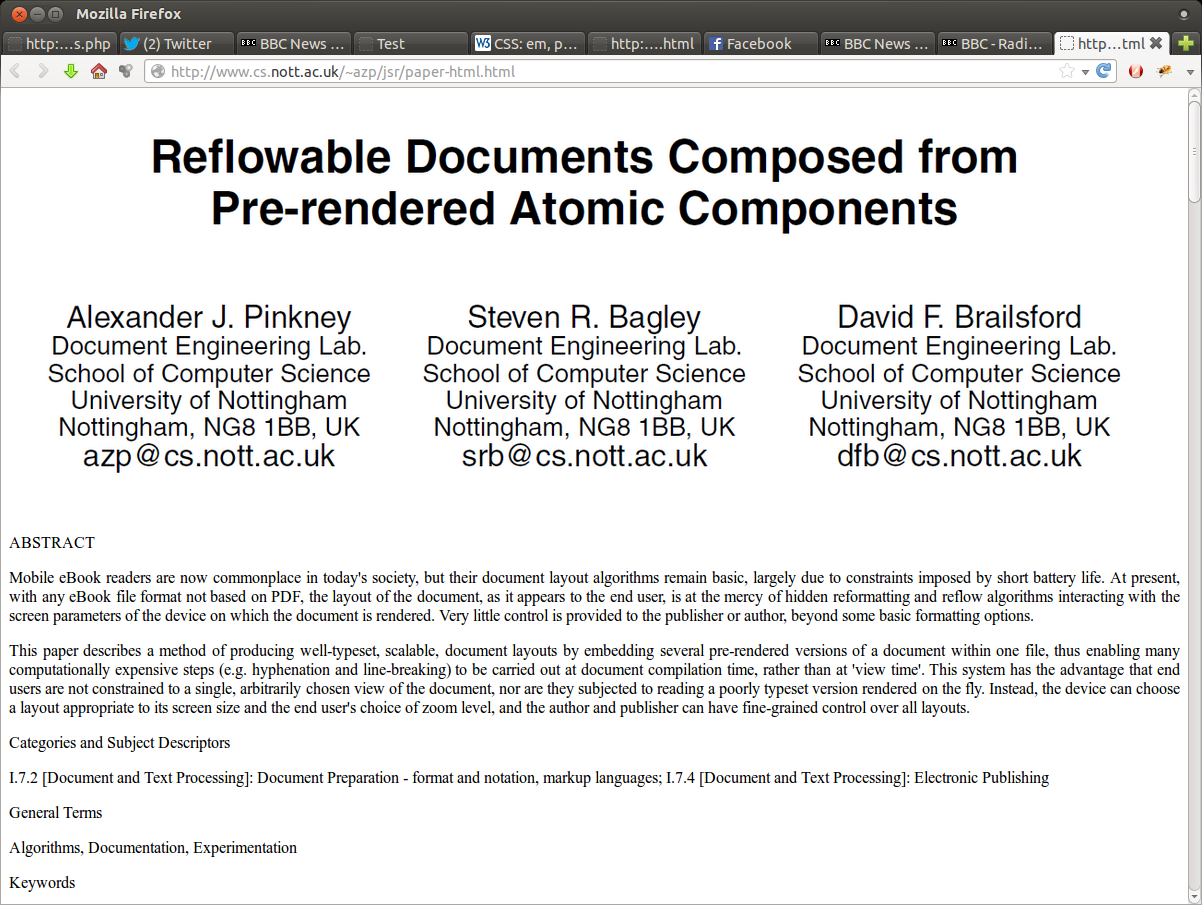
\includegraphics[trim=0in 0in 0in 1.2in, clip=true, width=0.47\textwidth]{gfx/html1}}\hspace{0.01\textwidth}
\fbox{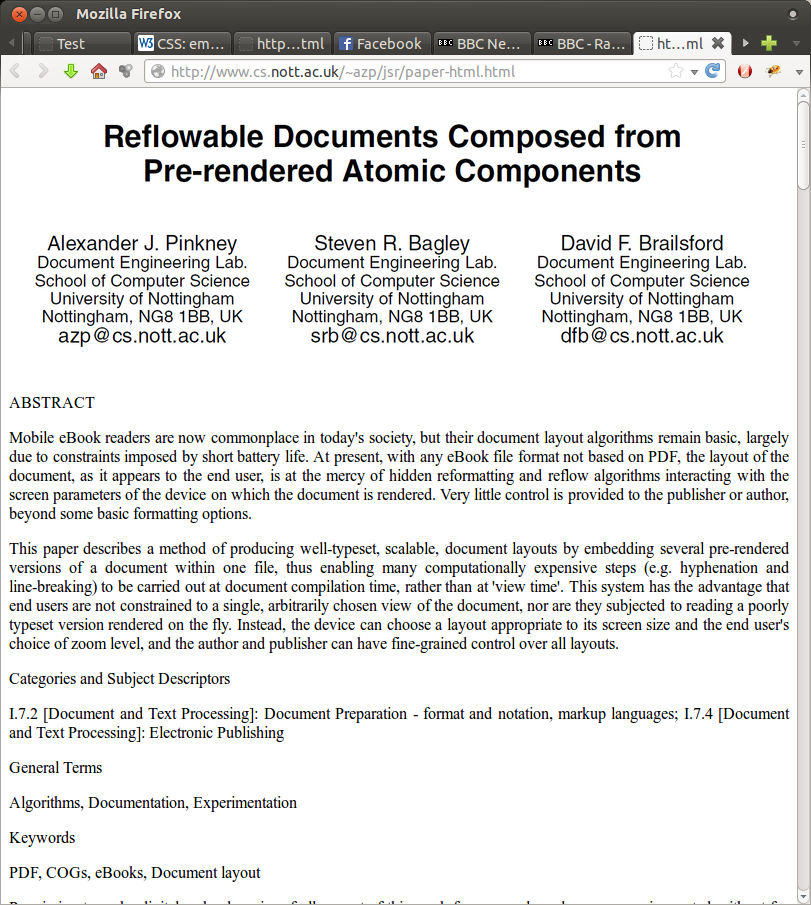
\includegraphics[trim=0in 0in 0in 1.2in, clip=true, width=0.47\textwidth]{gfx/html2}}

\vspace{0.2in}
\fbox{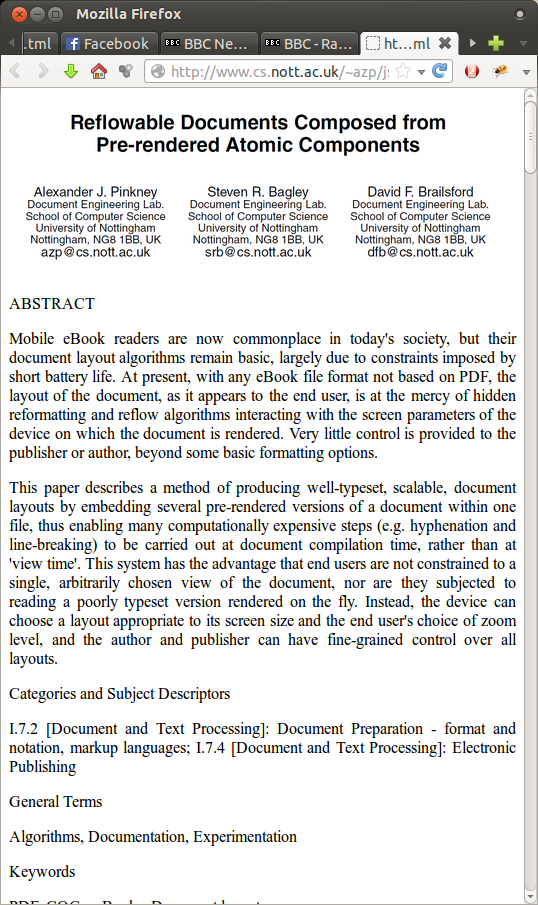
\includegraphics[trim=0in 0in 0in 1.2in, clip=true, width=0.47\textwidth]{gfx/html3}}\hspace{0.01\textwidth}
\fbox{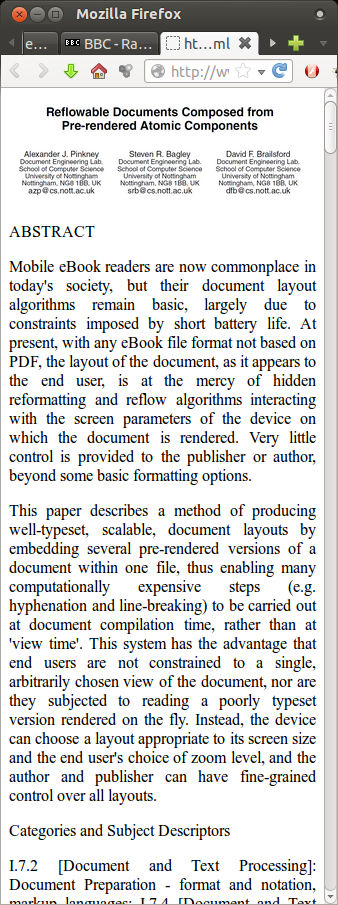
\includegraphics[trim=0in 0in 0in 1.2in, clip=true, width=0.47\textwidth]{gfx/html4}}
\end{center}
\caption[A document laid out by Mozilla Firefox]{\gls{html} version of \cite{Pinkney2011}, as rendered by Mozilla Firefox, scaled to fit multiple screen sizes. Though \gls{html} can stretch to any screen size, it tends to produce typographically inferior results, for example lines that are too long, or line breaking that results in extremely uneven spacing between adjacent lines.}
\label{fig:example-html}
\end{figure}

\section{Measures of Aesthetic Quality}
In their 2004 paper, Harrington et al.~\cite{Harrington2004} identified nine aesthetic measures for automated document layout. A number of these measures (alignment, regularity, uniform separation, white-space free-flow, uniformity) are inherently well satisfied by this system, due to its use of a grid to provide regular layout. 



%   - Greeking\\
%       - Default browser layout vs mine\\
%       - Look at \cite{Harrington2004} for some measures and say why mine is awesome\\
%   - some discussion of choices of galley widths for best performance


\section{Summary}
The malleable document system devised in this thesis was designed to be used for linear documents whose content is primarily text. Examples of such documents would be novels and scientific papers, but not reference books or graphic-heavy documents such as comics or children's picture books.

The layouts produced by this system are visually very similar to those of both newspapers and scientific papers, and can be flowed to fit virtually any page size. For smaller screen sizes, where single- or double-column spreads occur, the layouts closely resemble those of physical books and magazines.

%\todo{Sum up a bit better}
